\section{Dark Matter and CMB}
\subsection{Proof of existence of dark matter}

Similar to how the Hubble constant sets a scale to compare the age of the universe to, the critical density parameter does so for the actual density of the universe. Since information about stellar mass and distance is already available, it is possible to attempt to calculate the age of the universe using this. Hence this was done and it was obtained that $\Omega_{stars} = \frac{\rho_{stars}}{\rho_c}\rightarrow 0.01$.
\\
This means that the visible baryonic matter content of the universe is not enough to ensure that the universe's density approaches the critical value. Hence the theory of nucleosysnthesis was proposed, and demands that conventional material cannot contribute an entire critical density and in fact placed a limit on the baryonic density:

\begin{center}
    $0.021 \leq {\Omega_B}h^2 \leq 0.025$
\end{center}

Since the lower limit predicted is higher than observed, there must be more baryonic matter than observed in stars. This is true and had been confirmed by observation of galaxy rotation curves. Since galaxies have differential rotation curves it is expected that the circumferential velocity of stars evolves as $\frac{1}{\sqrt{R}}$, implying that it must reduce as distance from the centre of the galaxy increases. However on it was observed that the velocity remained approximately constant at larger radii, posing an evident contradiction. Since the circumferential velocity is also a function of mass enclosed between 0 to R it can be reasoned that the amount of mass increases along with radius, rather than stay constant as expected initially. This extra mass is what we call \textbf{dark matter}. 
\\
The calculated density of the dark matter halo comes out to be $\Omega_{halo} \approx 0.1$. It is expected that the dark matter is in the form of a spherical halo due to lack of any mechanism of collapse, owing to its extremely weak interaction.

\begin{figure}[H]
    \centering
    \includegraphics[width=0.8\textwidth]{figure6.jpg}
    \caption{The galaxy rotation curve of the galaxy NGC 6503 is shown here. Plots of the contributions from the three components, namely halo, disk and gas are also shown. The net result is a sum of the three.}
    \label{fig:curvesrotation}
\end{figure}

\subsection{Large Scale Structure}
Observations of galaxy clusters has lead to the conclusion that the density of hot gas component is 5 to 10 times higher than the density contribution form stars, which is also in agreement with their observed abundances.
\\
Observations of this hot gas have also enabled estimation of amount of dark matter present since the gravitational attraction from the cluster and surrounding gas is not enough to counter the thermal pressure from the gas. Hence the amount of dark matter can be estimated as:

\begin{center}
   $\frac{\Omega_B}{\Omega_0} \approx 0.065 h^{-\frac{3}{2}}$
\end{center}

Applying the nucleosysnthesis constraint gives the density parameter value as 0.4, suggesting the dark matter contribution is significantly higher than baryonic contribution. Further observation and analysis of the large scale structure of the universe and it anisotropies have cemented the idea that non-baryonic matter such as dark matter does indeed exist.

Finally measurement of the geometry of the universe was also carried out by some satellites (such as Planck) and have lead to the conclusion that \textbf{the universe is close to spatially flat} geometry, with $\Omega_0 \approx 0.3$ and $\Omega_{\Lambda} \approx 0.7$. This is also backed up by the theory if cosmological inflation.

\subsection{Nature of dark matter}
At present there is no clear idea of what constitutes dark matter, but there are some theoretical predictions from particle physics. One favourable dark matter candidate is the neutrino, assumed mass-less in cosmology but almost certainly has mass according to experiments being done currently. Neutrinos are extremely weakly interacting particles. There are three types of neutrinos: electron neutrino, muon neutrino and tau neutrino and present experiments place the latter two on a higher probability of being a dark matter candidate.
\\
Since the mass of neutrinos haven't been clearly determined, light and heavy neutrinos could lead to different kinds of dark matter namely hot dark matter (relativistic) and cold dark matter respectively.

Other particles proposed as dark matter candidates are the Light Supersymmetric Particle (LSP) and Weakly Interacting Massive Particles (WIMP).

\subsection{Cosmic Microwave Background}

\begin{figure}[H]
    \centering
    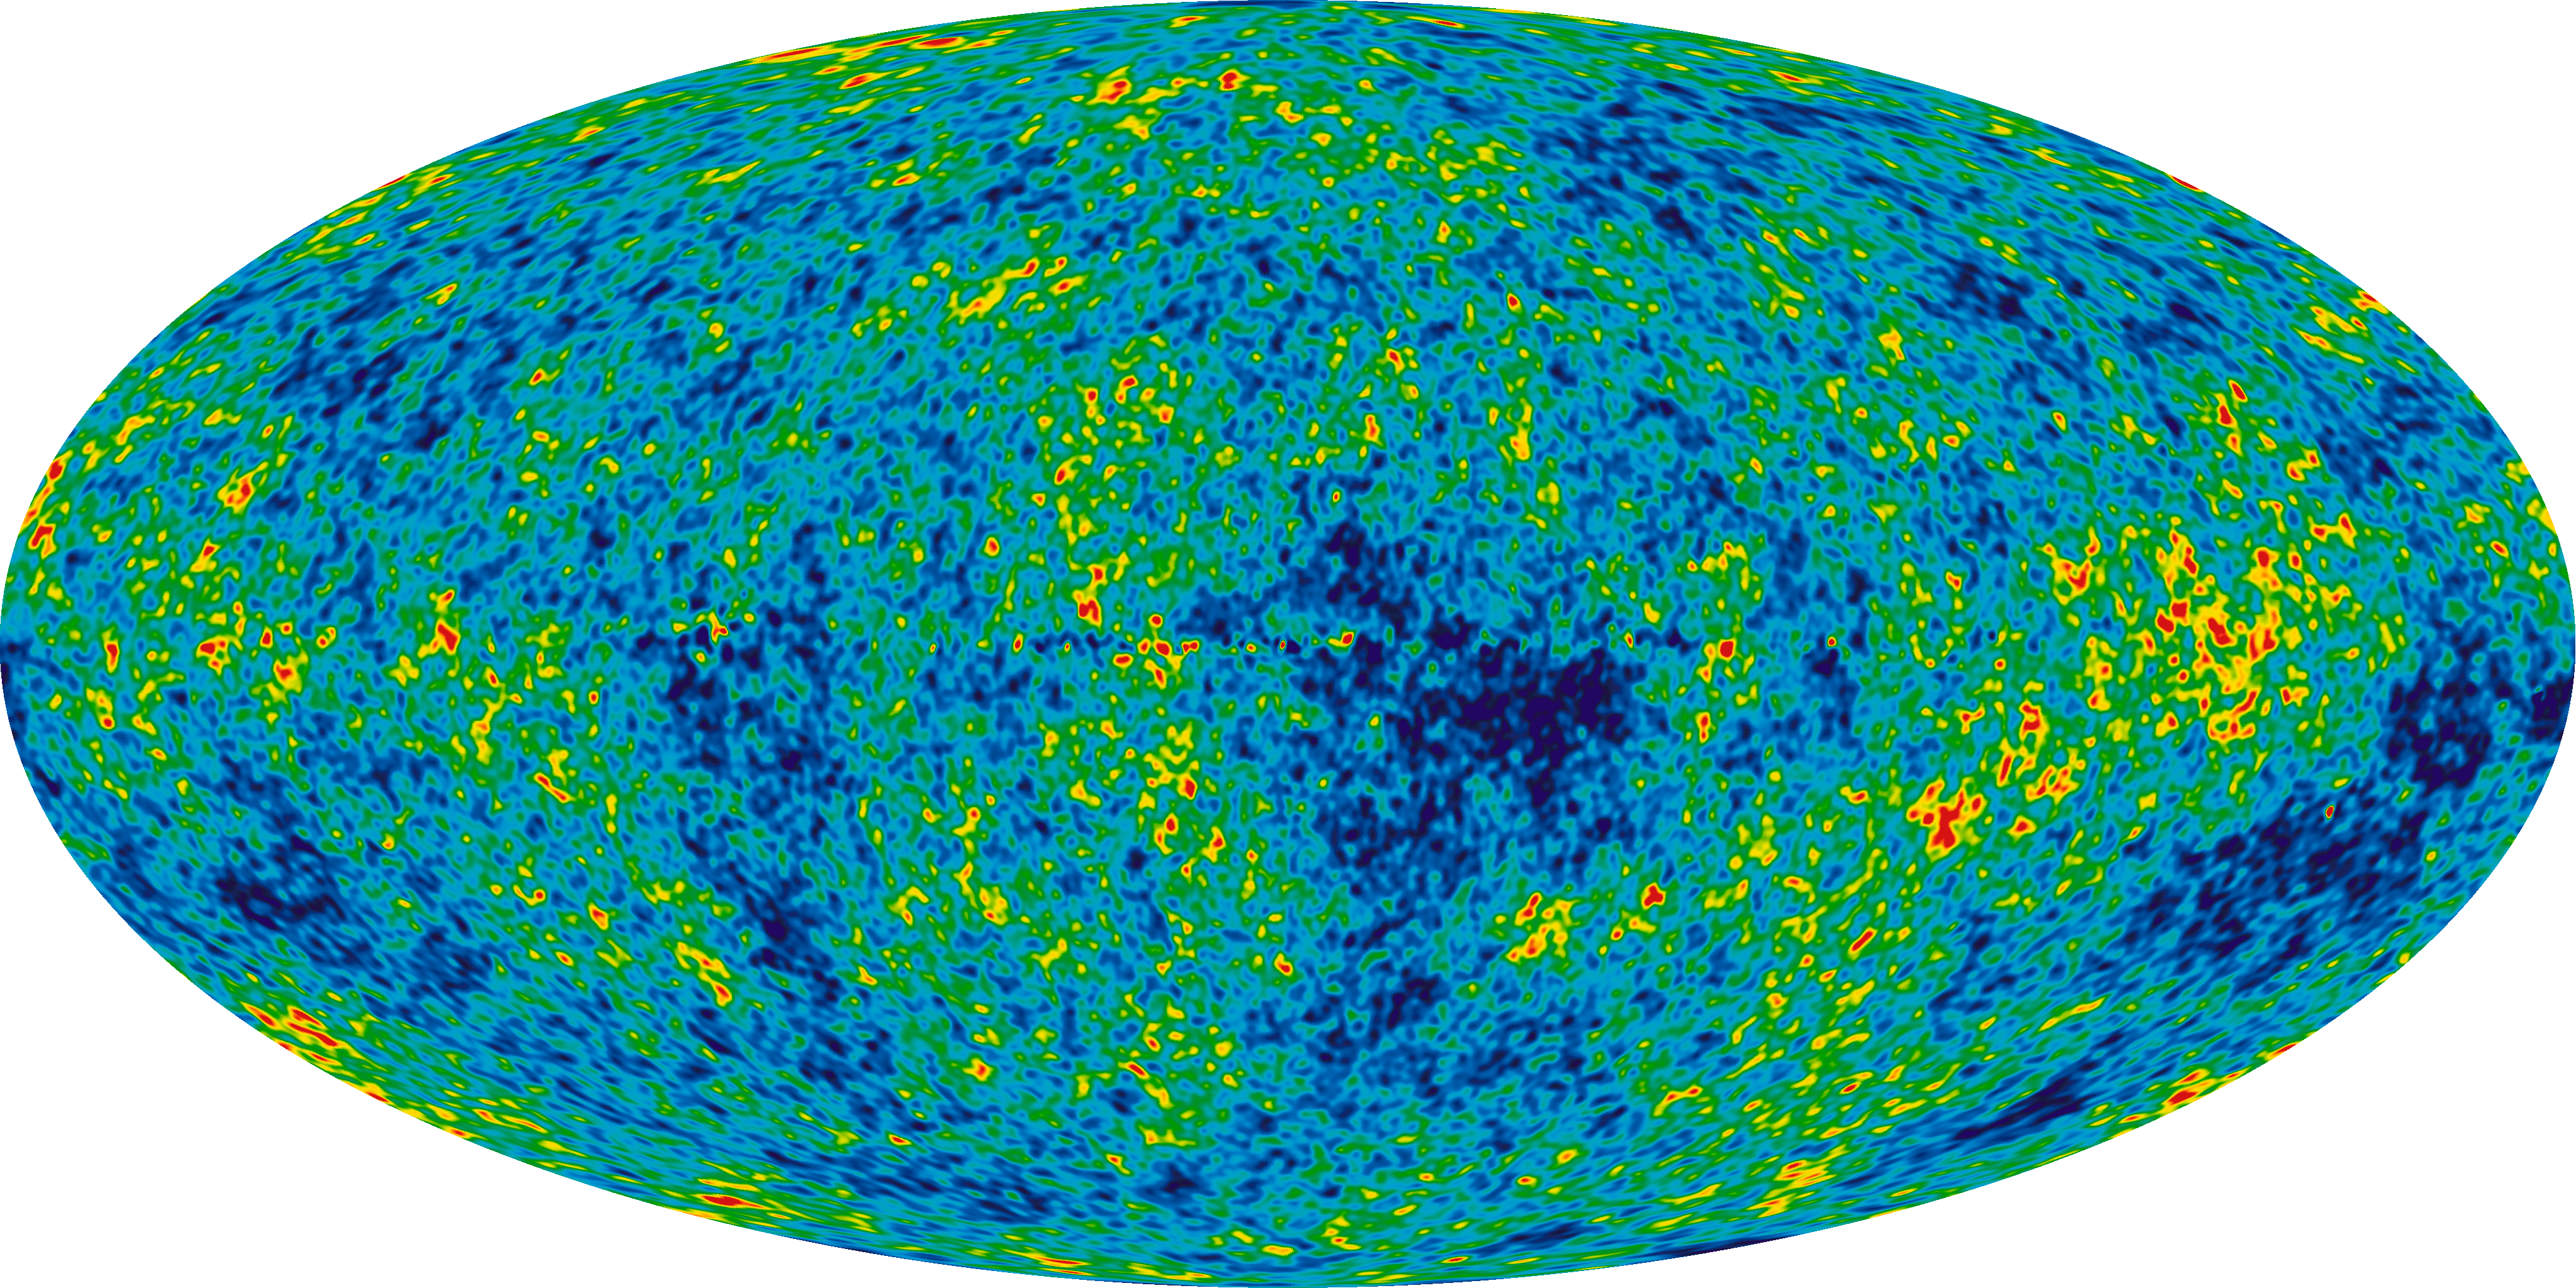
\includegraphics[width=0.8\textwidth]{figure 7.png}
    \caption{The cosmic microwave background}
    \label{fig:CMB}
\end{figure}

The CMB behaves similar to a black body with a temperature of $2.725 \pm 0.001 k$. When the energy corresponding to it is converted and written in terms of the critical density it come ou to be $\Omega_{rad} = 2.47$ x $10^{-5} h^{-2}$, which implies that it contributes to a small fraction of the universe's density.
\\
Stefan's law states that
\begin{center}
    $\epsilon_{rad} = \rho_{rad}c^2 = \frac{{\pi}^2{k_B}^4}{15{\hbar}^3c^3}T^4$
\end{center}

Since $\rho_{rad}$ evolves as $\frac{1}{a^4}$, it turns out that $T \propto \frac{1}{a}$, which means that the temperature of the universe must have been arbitrarily large in its beginning stages. Another element associated with this concept is the conservation of particle number. Given that the interactions between baryons and photons are negligible, their number density must be preserved as the universe expands. Hence 

\begin{center}
    $n_{\gamma} = \frac{\epsilon_{rad}}{E_{rad}} = 3.7$ x $10^8 m^{-3}$
\end{center}

\begin{center}
    $n_{B} = \frac{\epsilon_{B}}{E_{B}} = 0.25 m^{-3}$ 
\end{center}

The smaller number of baryons is due to the fact that their mass-energy is much higher, despite having higher energy density than photons.
\\
The origin of the CMB can be understood by considering the interaction between atoms and photons in the early universe. When the temperature was much higher, say $3$x$10^6 K$, the average energy of photons is enough to ionize the hydrogen atom from its ground state,which means that atoms could not be formed. Hence the early universe was a sea of electrons, protons and photons.
When the universe eventually cooled down, the average energy of photons fell and were not enough to ionize hydrogen completely. This event is called \textbf{decoupling}, wherein the universe suddenly changed from being completely opaque to transparent.
\\
A crude estimate can be obtained by comparing the average energy of photons $(3k_{B}T)$ to the ionization energy of hydrogen which is 13.6 eV. Dividing these quantities gives the temperature as 50000K. 
This is actually incorrect, even for an estimate. The reason is that ionization of hydrogen will still continue when the average energy if photons is below 13.6 eV due to the presence of high energy photons in the tail of the Boltzmann distribution. Taking that into account gives a better estimate:

\begin{center}
    $T_{dec} = 7400 K$
\end{center}

There is yet another phenomena which needs to be taken into account, which is \textbf{recombination}.Recombination refers to the time period when the protons and electrons first combined to form atoms. Since this process is not instantaneous it does not coincide with decoupling. Since decoupling cannot happen before recombination happens, this makes the temperature obtain earlier higher than the actual value. This new value can be obtained by using the Saha equation:

\begin{equation}
    \frac{1-X}{X} \approx 3.8\frac{n_B}{n_{\gamma}}(\frac{k_{B}T}{m_{e}c^2})^{\frac{3}{2}}e^{\frac{E_0}{k_{B}T}}
\end{equation}

where X is the protons to baryons, indicating the amount of ionization.This implies that the ionization will be large is the RHS of the equation is small. Recombination is defined to correspond to $X = 0.1$, i.e the process is 90 percent complete. Using this to solve the equation gives the temperature of the universe at decoupling to be \textbf{3600 K}.
\\
The fact that the CMB is a black body radiation is well explained by this model as the photons and baryons were in thermal equilibrium before decoupling. Since then the photons would travel without interruption and reach us from the surface of last scattering.
